\documentclass[a4paper,12pt]{article}
\usepackage[14pt]{extsizes}
\usepackage[utf8]{inputenc}
\usepackage[russian]{babel}
\usepackage{glossaries}
\usepackage{graphicx}
\usepackage{float}
\usepackage{amsfonts}
\usepackage[left=3cm,right=1cm,top=1cm,bottom=2cm]{geometry}
\graphicspath{ {./pictures/} }
\usepackage{setspace}
%%\renewcommand{\rmdefault}{ftm} % Times New Roman

\onehalfspacing

\makeglossaries

\begin{document}

\tableofcontents

\section*{Аннотация}
В рамках данной работы реализована серверная часть системы управления соревнованиями роботов.

\section{Введение}
В последнее время, в связи с развитием микроконтроллеров и популяризацией таких проектов как Arduino \cite{web:arduino}, особенную популярность в мире набирают чемпионаты по программированию роботов.
Такие как например Robotics Tournament \cite{web:robotournament} проводимый центром развития робототехники на базе Дальневосточного Федерального Университета. DARPA Robotics Challenge \cite{web:drc} проводимый американской компанией DARPA по проектированию гуманоидных роботов. И многие другие. 

Количество участников на таких соревнованиях иногда достигает колоссальных масштабов, что сильно сказывается на времени их проведения.
Соответственно встает вопрос, об автоматизации процесса проведения таких соревнований.

\subsection{Глоссарий}
\newglossaryentry{ee}{name=Исполняющая единица, description={Аппаратная подвижная платформа способная запускать пользовательский код}} 

\printglossaries

\subsection{Описание предметной области}
В современном мире, область применения робототехники в различных сферах деятельности человека очень широка и не перестает расти. Применение роботов позволяет значительно снизить участие человека в тяжелой и опасной работе. Например, работа в оборонных, химических, атомных сферах, тушение пожаров без помощи оператора, выполнение спасательных операций или передвижение по заранее неизвестной местности. Постепенно роботы входят и в обычную жизнь человека.

Для стимулирования и продвижения исследований в этой области, различные крупные компании, заинтересованные в робототехнике, такие как например DARPA, проводят свои собственные соревновательные турниры - Darpa Robotic Challenge \cite{web:drc}. В этих соревнованиях принимало участие до 23 команд из разных стран мира \cite{web:darpa-finals}.

Электронные и аппаратные компоненты для создания роботов становятся все доступнее, что обуславливает популяризацию любительской робототехники. Появляются учебные центры, специализирующиеся на обучении детей школьного возраста программированию и строительству роботов. Самые крупные из них это "Лига роботов" \cite{web:ligarobotov} имеющая центры по всей стране, и "Центр развития роботехники" \cite{web:robocentr} имеющий несколько филиалов на территории дальнего востока. Последний, в частности, проводит локальные соревнования по строительству роботов - "Robotics Tournament" \cite{web:robotournament}. В 2018 году в этом соревновании приняли участие 31 команда со всего дальнего востока \cite{web:robotournament-finals}.

При автоматизации учебного процесса все чаще находят место тестирующие системы, которые также применяются в спортивном программировании для автоматизации проведения соревнований, а также проверки работоспособности программ.

\subsection{Неформальная постановка задачи}
В рамках работы требуется реализовать следующие возможности:
\begin{enumerate}
    \item Создавать турниры типа "Соревнования роботов"
    \item Редактировать список доступных исполняющих едениц.
    \item Загружать и запускать решения участников на исполняющей еденице.
    \item Собирать и анализировать резульаты запуска решений участников.
    \item Формировать и просматрировать результаты турниров по правилам характерным для соревнований роботов;
\end{enumerate}

\subsection{Обзор конкурирующих решений}
\subsubsection{The Robot Programming Network}
The Robot Programming Network - это инициатива по созданию сети учебных лабораторий робототехники с возможностями удаленного программирования. Он состоит из материалов открытого онлайн-курса и онлайн-серверов, которые готовы выполнять и тестировать программы, написанные удаленными студентами. 

Онлайн материалы включают в себя вводные учебные модули по программированию роботов, мобильной робототехнике и гуманоидам, нацеленные на изучение базовых понятий в науке, технике, инженерии и математике (STEM) и углубленных навыков программирования. Студенты имеют доступ к хостам онлайн-сервера, где они отправляют и запускают свой программный код на лету. \cite{web:rpn}

\begin{figure}[H]
    \centering
    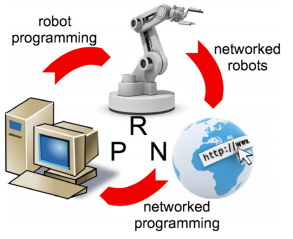
\includegraphics{pictures/RPNConcept.png}
    \caption{Концепт системы Robot Programming Network}
    \label{fig:rpn_concept}
\end{figure}

Плюсы данной платформы:
\begin{enumerate}
    \item Перед отправкой решения есть возможность протестировать его в виртуальной среде
    \item Большое количество обучающих материалов и онлайн курсов
    \item Отсутствует обратная связь с роботом
\end{enumerate}

Минусы данной платформы:
\begin{enumerate}
    \item Отсутствует возможность автоматической проверки выполнения поставленных задач
    \item Закрытый исходный код
\end{enumerate}

\subsubsection{The Robotarium}
Robotarium используется в качестве исследовательского испытательного стенда для роботов, главная цель Роботариума - снизить барьер входа в многоагентную робототехнику и обеспечить доступ к современному испытательному оборудованию для исследователей по всему миру. Поэтому удаленный доступ является неотъемлемой частью дизайна Robotarium и в настоящее время реализуется через общедоступный веб-интерфейс, который дает пользователям возможность тестировать различные алгоритмы с несколькими роботами. Обеспечение доступности роботизированного оборудования в режиме онлайн требует от Роботариума решения ряда задач, включая надежную и безопасную долгосрочную работу больших групп роботов с минимальным вмешательством оператора.

Плюсы данной платформы:
\begin{enumerate}
    \item Есть возможность тестирования многоагентных алгоримтов
\end{enumerate}

Минусы данной платформы:
\begin{enumerate}
    \item Отсутствует возможность организации пользовательских турниров
    \item Закрытый исходный код
\end{enumerate}

\subsubsection{Сравнительная таблица}
\begin{table}[H]
    \begin{tabular}{|p{5cm}|c|c|c|}
    \hline
    Признак/Платформа & CATS & Robot Programming Network & The Robotarium \\
    \hline
    Отслеживание исполнения программы & + & - & + \\
    \hline
    Запуск пользовательского кода & + & + & + \\
    \hline
    Возможность организовывать пользовательские турниры & + & - & - \\
    \hline
    Свобода в выборе ЯП & + & - & - \\
    \hline
    \end{tabular}
    \caption{Сравнительная таблица конкурирующих решений}
    \label{tab:my_label}
\end{table}

\section{Архитектура}
Разработанная мною система подрзарделяется на несколько основных модулей. И представляет из себя программно-аппаратный комплекс. 

\begin{figure}[H]
    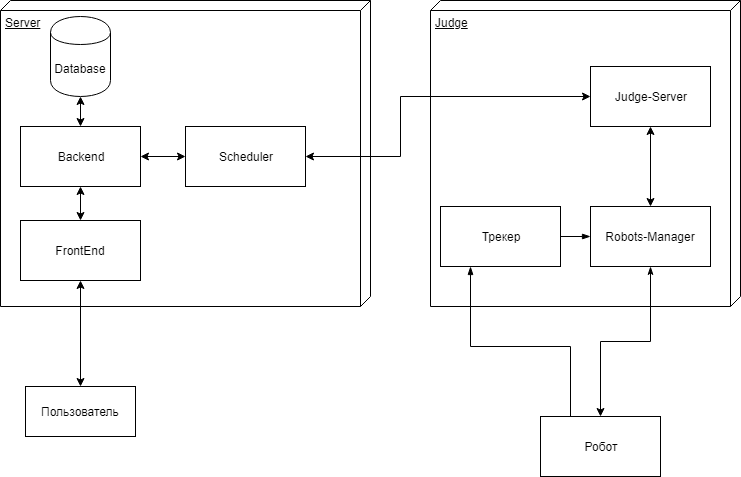
\includegraphics[width=\textwidth]{pictures/Architecture.png}
    \caption{Программная архитектура комлпекса}
    \label{fig:arch_diagram}
\end{figure}

\subsection{Архитектура модуля Main}
Архитектура модуля Main подразделяется на веб-интерфейс для взаимодействия с пользователем, модуль Backend осуществляющий взаимодействие с базой данных и модуля Scheduler организующего планирование запуска решений участников.

\subsubsection{Веб интерфейс}
Веб-интерфейс является основным инструментом для взаимодействия с комплексом. Он представляет из себя одностраничное веб-приложение написанное с использованием библиотеки React \cite{web:react}. 

\subsubsection{Backend}
Модуль Backend представляет из себя веб сервер написанный на языке PHP с использованием фреймворка Laravel \cite{web:laravel}.

\subsubsection{Scheduler}
Модуль Scheduler предназначен для планирования запусков решений участников, согласно выбранной пользователем турнирной таблицы. 

\subsubsection{База данных}
В базе данных хранится информация о проводимых турнирах, исходный код участников, пакеты задач и результаты тестирования.

\subsection{Архитектура модуля Judge}
Модуль Judge является программно-аппаратным комплексом и делится на веб сервер состоящий из модуля Judge-Server и Robots-Manager и трекера, который служит для отслеживания робота в пространстве.

\subsubsection{Judge-Server}
Это веб-сервер отвечающий за непосредственный запуск решений участников на роботах, и сбор информации о прохождении задания. 

\subsubsection{Robots-Manager}
Robots-Manager - программный модуль отвечающий за взаимодействие с пулом исполняющих агентов. В его задачи входит:
\begin{enumerate}
    \item Загрузка пользовательского кода в испольняющую еденицу
    \item Отправка команд роботу
    \item Сбор телеметрии
\end{enumerate}

\subsubsection{Трекер}
Трекер - программно аппаратный модуль, в задачи которого входит отслеживание перемещения агентов на площадке для тестов. 

\section{Спецификация данных}

\subsection{База данных}

\begin{figure}[H]
    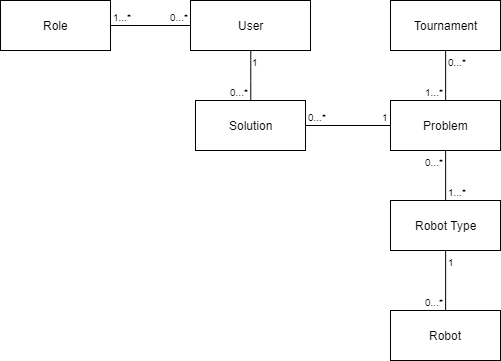
\includegraphics[width=\textwidth]{pictures/database_diagram.png}
    \caption{Диаграмма таблиц базы данных}
    \label{fig:db_diagram}
\end{figure}

На рисунке \ref{fig:db_diagram} изображена диаграмма отношения таблиц базы данных. 
Рассмотрим каждую из них по отдельности

\subsubsection{Role}
Для разграничения доступа пользователей к некоторым функциям системы, каждому пользователю привязывается соответствующая роль. Например, роль Jury позволяет пользователю добавлять в турнир новые задачи, а также просматривать решения участникав. Роль Admin предоставляет полные привилегии доступа к системе. 

\subsubsection{User}
Описывает пользователя системы.
У каждого пользователя может быть указано:
\begin{enumerate}
    \item Никнейм
    \item Электронная почта
    \item Хеш пароля
    \item Фамилия
    \item Имя
\end{enumerate}
В целях безопасности, в базе данных хранится хеш (SHA-256) пароля пользователя с солью. 

\subsubsection{Problem}
Одна из главных таблиц, описывающая задачу в системе.
Задача описывается следующими полями:
\begin{enumerate}
    \item Имя
    \item Типы роботов, допустимых для решения задачи
    \item Ссылка на репозиторий git
\end{enumerate}
Чтобы уменьшить количество хранимой в базе информации, было решено хранить пакет задачи в репозиториях git. Помимо сокращения объема базы данных, это позволяет пользователям с легкостью исправлять загруженные задачи, использую систему Continuous Integration (CI). Также позволяя переиспользовать код между различными задачами, используя встроенную в git систему подмодулей.

\subsubsection{Solution}
Описывает отправленное участников решение. Таблица, помимо указанных на рис. \ref{fig:db_diagram} отношений, имеет следующие поля:
\begin{enumerate}
    \item Время отправки решения
    \item Ссылка на репозиторий git
    \item Идентификатор коммита
\end{enumerate}

Каждая попытка отправленная участником на тестирование, не должна меняться после отправки. Для этого, в попытку добавляется идентификатор коммита. В случае если участник обновил решение и хочет его перетестировать, ему необходимо снова отправить решение свое решение с указанием нового идентификатора коммита. 

\subsubsection{RobotType}
Указывает тип исполняемой еденицы. В системе может быть зарегистрированы роботы разных типов, пригодных для выполнения специфических задач. К примеру это могут быть колесные или гусеничные платформы, летающие дроны, шагающие роботы. 

\subsubsection{Robot}
Описывает зарегистрированного в системе робота.

\subsubsection{Tournament}
Турнир созданный пользователем.

\section{Функциональные требования}
Система должна позволять участникам:
\begin{enumerate}
    \item Загружать своим решения
    \item Просматривать результаты тестирования
    \item Просматривать результаты тестирования
\end{enumerate}
Система должна позволять жюри, включая предыдущие требования:
\begin{enumerate}
    \item Добавлять новые задачи
    \begin{enumerate}
        \item Выбирать пул роботов, на котором следует запускать решения участников
        \item Ограничивать количество участников для одного запуска
        \item Загружать "контроллер" в задачу, или импортировать из уже загруженных в систему.
    \end{enumerate}
    \item Сохранять и просматривать результаты запуска решения участника
    \item Генерировать и просматривать турнирную таблицу
\end{enumerate}

\section{Требования к интерфейсу}
В интерфейса участника необходимо иметь возможность:
\begin{itemize}
    \item Посмотреть список турниров.
    \item Посмотреть список отправленных решений в каждый турнир.
    \item Посмотреть результаты тестирования.
\end{itemize}

При просмотре результата тестирования, требуется отобразить:
\begin{itemize}
    \item Вердикт решения участника.
    \item Время отправки решения.
    \item Автора решения.
    \item Ссылку на репозиторий.
    \item Hash id коммита.
    \item Комментарий контроллера (опционально)
\end{itemize}

При просмотре списка турниров, требуется отобразить:
\begin{itemize}
    \item Имя турнира.
    \item Время начала и окончания турнира.
    \item Время до начала турнира.
    \item Правила турнира.
\end{itemize}

При создании нового турнира, необходимо иметь возможность:
\begin{itemize}
    \item Указать время начала и время окончания турнира.
    \item Указать правила проведения турнира и тип турнирной сетки.
    \item Указать наименование турнира.
\end{itemize}

При редактировании списка задач в турнире, требуется возможность:
\begin{itemize}
    \item Добавить новую задачу.
    \item Удалить задачу. 
    \item Изменить статус задачи на:
    \begin{itemize}
        \item \verb+OK+ - задача отображается, и в неё можно загружать решения.
        \item \verb+Hidden+ - задача скрыта в турнире.
        \item \verb+Suspended+ - прекратить проверку решений для данной задачи.
    \end{itemize}
\end{itemize}

При просмотре списка задач участником в турнире, требуется иметь возможность:
\begin{itemize}
    \item Посмотреть описание задачи.
    \item Посмотреть список отправленных решений для данной задачи.
\end{itemize}

При просмотре турнирной таблицы, требуется:
\begin{itemize}
    \item Отобразить схему турнирной таблицы.
    \item Отобразить результаты прошедших состязаний.
\end{itemize}

\section{Проект}
\subsection{Средства реализации}
При разработке использовался фреймворк Laravel 5.5 и язык программирования PHP. В качестве базы данных я выбрал PostgresQL 10. Laravel является одним из самых популярных фреймворком для разработки на языке PHP. А следовательно имеет большее компьюнити, и большее количество обучающей информации. 

\section{Модули и алгоритмы}
\subsection{Модуль RATS::Common}
Этот модуль является общим для модулей \verb+RATS::Main+ и \verb+RATS::Judge+, и содержит в себе функции и классы общие для каждых из двух модулей. 
\subsubsection{Модуль RATS::Common::GitUtils}
Модуль предзначенный для работы с git репозиториями. В его задачи входит клонирование репозиториев, их кеширование и другая работа с ними. Все задачи и решения участников предлагается хранить не локально на сервере, а в виде гит репозиториев. Так как git предполагается использовать как на главном сервере, так и на серверах Judge, данный модуль было решено сделать общим, и вынести в подмодуль RATS::Common.

По умолчанию, репозитории должны быть открытыми. Если пользователь хочет использовать приватный репозиторий, то он должен быть размещен в хранилище GitHub \cite{web:github}. Пользователь должен добавить в свой приватный репозиторий коллаборатора - специального пользователя, из под которого система будет получать доступ. 

Модуль имеет слуедуюшие функции:
\begin{itemize}
    \item \verb+git_clone(string repo)+: Функция принимает на вход ссылку на гит репозиторий и клонирует его в локальное хранилище. Если репозиторий уже кеширован, то функция просто выполнит git fetch. Если репозиторий не существует, сгенерируется исключение.
    \item \verb+git_checkout(string repo, string commit_hash)+: Переключает репозиторий на данный коммит. Если репозиторий не был кеширован, вызовоется функция git\_clone для данного репозитория. Если данного коммита не существует, сгенерируется исключение. 
    \item \verb+git_remove(string repo)+: Удаляет репозиторий из кеша. Если репозитория не существовало, то данный факт проигнорируется. 
    \item \verb+git_get_path(string repo)+: Возвращает путь к корню кешированного репозитория. Если репозитория не существует, вызовется функция \verb+git_clone+. 
    \item \verb+git_check(string repo, string commit_hash)+: Проверяет, что репозиторий по ссылке и коммит с таким хешем в нем действительно существует. 
\end{itemize}

\subsubsection{Модуль RATS::Common::Problem}
В этот модуль вынесены общие для двух модулей функции для работы с задачей. В первую очередь это функции для работы с репозиторием задачи. Модуль имеет следующие функции:

\begin{itemize}
    \item \verb+get_info(int problem_id)+: Функция возвращает структуру с описанием задачи. 
    \begin{enumerate}
        \item \verb+string title+: Название задачи.
        \item \verb+blob info_template+: Файл шаблона с описанием задачи.
        \item \verb+int robot_type+: Тип робота, для которого написана задача.
        \item \verb+string get_bundle_path+: Путь к ros бандлу задачи.
    \end{enumerate}
\end{itemize}

\subsubsection{Модуль RATS::Common::Solution}

\subsection{Модуль RATS::Main}
\subsubsection{Модуль RATS::Main::Problem}
Программный модуль отвечающий за взаимодействие с задачами.
Каждая задача характеризуется описанием в виде HTML страницы, или в виде шаблона для шаблонизатора Blade.
И специальной программой - контроллером, в задачи который входит оценка действия программы пользователя и выставление очков за прохождение. Описание контроллера будет в части \verb+RATS::Judge::Problem+

Состоит из следующих функций: 

\begin{itemize}
    \item \verb+create_problem(string title, string repo)+: Функция создающая задачу и возвращающая её id. Функция на вход принимает ссылку на git репозиторий с задачей. Если задача с таким репозиторием уже существовала, функция геренрирует исключение.
    \item \verb+remove_problem(int problem_id)+: Удаляет задачу из системы. Принимает на вход id задачи. Если задачи с таким id не существовует, функция генерирует исключение.
\end{itemize}

\subsubsection{Модуль RATS::Main::Tournament}
Модудь для управления турнирами в системе. 

\begin{itemize}
    \item \verb+create_tournament(string title)+: Создает турнир с заданным именем.
    \item \verb+remove_tournament(int tournament_id, bool force)+:  Удаляет турнир с заданным id. Если турнира с таким id не существует, функция генерирует исключение. Если турнир имеет в себе отправленные решения участников, функция сгенерирует исключение. Для того чтобы полностью удалить турнир со всеми решениями участников, нужно вызвать функция с флагом force. В результате турнир будет удален со всеми решениями участников.
\end{itemize}

Каждый турнир характеризуется временем начала и временем конца принятия решений участников. Решения принимаются только в этом промежутке. Во всем остальных случаях будет сгенерировано исключение. Существует возможность указать неограниченное время принятия решений.

\subsubsection{Модуль RATS::Main::Solution}
Данный модуль отвечает за работу с решениями пользователей. Имеет следующие функции:

\begin{itemize}
    \item \verb+create_solution(int user_id, int problem_tournament_id, string repo, string hash)+: Добавляет решение участника в систему. Если такого пользователя нет, функция генерирует исключение.
    \item \verb+remove_solution(int solution_id)+: Удаляет решение пользователя из системы. Если решения с таким id не существует, функция генерирует исключение.
    \item \verb+get_solution_info(int solution_id)+: Возвращает структуру с описанием решения пользователя. Структура имеет следующие поля:
    \begin{enumerate}
        \item \verb+TimeStamp сreate_date+ - дата и время создания решения.
        \item \verb+int problem_id+ - id задачи к которой относится решение.
        \item \verb+int user_id+ - пользователь создавший решение.
        \item \verb+string git_repo+ - ссылка на git репозиторий решения.
        \item \verb+string commit_hash+ - хеш коммита решения.
        \item \verb+int status+ - статус решения участника, может принимать следующие значения:
        \begin{enumerate}
            \item \verb+registered+ - статус, который принимает решение сразу после добавления.
            \item \verb+install+ - решение устанавливается на RATS::judge. 
            \item \verb+accepted+ - решение принято.
            \item \verb+runtime_error+ - решение сгенерировало исключение во время выполнения.
            \item \verb+security_violation+ - решение было остановлено из за нарушения протоколов безопасности.
            \item \verb+compile_error+ - при сборке решения возникли ошибки.
            \item \verb+wrong_repo+ - ссылка на репозиторий решения не действительна.
        \end{enumerate}
    \end{enumerate}
\end{itemize}

\subsubsection{Модуль RATS::Main::User}
Модуль для управления пользователями. 

\begin{itemize}
    \item \verb+create_user(string name, string password)+ - Создает нового пользователя с заданным именем и паролем.
    \item \verb+remove_user(int id)+ - Удаляет пользователя с заданным id. 
\end{itemize}

\subsubsection{RATS::Main::Judges}
Этот модуль отвечает за взаимодействие с \verb+RATS::Judge+, их добавление и настройки. Взаимодействие с \verb+RATS::Judge+ организовано посредством WebApi. У каждого запущенного инстанса \verb+RATS::Judge+ существует уникальный идентификатор который задается в конфигурации \verb+RATS::Judge+. Регистрация нового инстанса происходит через Web интерфейс. Для этого основной сервер и инстансы \verb+RATS::Judge+ должны находится в одной локальной сети.

Протокол взаимодействия \verb+RATS::Main+ и \verb+RATS::Judges+ выглядит следующим образом:

\begin{itemize}
    \item Регистрация \verb+RATS::Judge+:
    
    Основной сервер посылает broadcast сообщение на порт 4573. Все получившие данные сообщения судьи отправляют в ответ свои идентификаторы. После чего они могут быть зарегистрированы в системе. Судьи в свою очередь получают IP адрес главного сервера, чтобы обращаться к нему за решениями участников.
    
    \item Отправка решения на проверку.
    
    RATS::Judge может принимать несколько состояний:
    \begin{itemize}
        \item \verb+greedy+ \verb+RATS::Judge+ сам отправляет запрос на сервер за новыми решениями участников, которые нужно проверить. Данный режим хорош для автоматической распределения нагрузки. 
        \item \verb+await+ - режим ожидания комманд, \verb+Judge+ проверяет только те задачи, которые ему направил главный сервер. Сам judge не отправляет никаких запросов главному серверу. 
        \item \verb+suspend+ - \verb+Judge+ не принимает запросы на проверку от главного сервера. 
    \end{itemize}
    
    \item \verb+Heartbeat+
    
    Для того чтобы поддерживать информация о всех инстаснах \verb+RATS::Judge+, они с некоторым промежутком времени отправляют пакет под названием Heartbeat, сигнализирующий о том, что судья еще жив и готов принимать решения.
\end{itemize}

\subsection{Модуль RATS::Judge}
Данный программный модуль запускается на площадках с роботами и отвечает за загрузку, запуск, контроль и сбор информации о решении пользователя.

\subsubsection{Модуль RATS::Judge::RobotsManager}
Этот модуль отвечает за поддержание и организацию работы с роботоами. В его задачи входит:

\begin{enumerate}
    \item Поиск и подключение роботов.
    \item Хранение и управление списком подключенных роботов.
    \item Обновление их состояния.
    \item Обновление программного обеспечения.
    \item Удаленное управление.
    \item Трекинг положения.
\end{enumerate}

За каждую из задач отвечает свой подмодуль. Рассмотрим каждый из них по отдельности.

\subsubsection{Модуль RATS::Judge::Robot}
Каждый тип робота описывается классом \verb+RATS::Judge::Robot<Type>+ унаследованным от базового класса \verb+RATS::Judge::RobotBase+.

\subsubsection{Модуль RATS::Judge::Tracker}
Для того чтобы отслеживать положение каждого робота на площадке, был создан модуль \verb+RATS::Judge::Tracker+.

Определение позиции каждого робота происходит визуальным методом. Сверху площадки установлена камера, которая направлена вниз. К каждому робота прикреплена уникальная графическая метка. Находя эту метку на изображении можно определить местоположение робота на площадке.

Для реализации этого подхода была использована популярная и открытая библиотека компьютерного зрения OpenCV. В ней уже были реализованы необходимые методы для распознования меток. Для нахождения метки я использовал метод сопоставления ключевых точек.

Существует множество различных методов для нахождения ключевых точек, наиболее популярные из них - это методы SURF, SIFT, AKAZE, ORB и др. Главным приоритетом для выбора метода, была скорость и стабильность работы. Роботы могут довольно быстро перемещаться по площадке, поэтому требуется обеспечить скорость распознования примерно в 20 кадров в секунду, чтобы алгоритмы контроля робота могли своевременно реагировать на изменения положения. 

Было проведено тестирование каждого из этих методов и замерил среднее количество времени требуемое на обработку одного кадра, разрешением 1680x1050. Замеры производились на компьютере со следующими характеристиками: 
CPU Intel Core i7 7550, 16GB DDR3 RAM, NVidia GTX1080Ti.

\begin{table}[H]
    \centering
    \begin{tabular}{|p{5cm}|c|}
    \hline
    Метод & Время \\
    \hline
    AKAZE & 113мс \\
    \hline
    AGAST & 142 \\
    \hline
    BRISK & 76мс \\
    \hline
    ORB & 53мс \\
    \hline
    SURF & 109мс \\
    \hline
    SIFT & 27мс \\
    \hline
    \end{tabular}
    \caption{Сравнительная таблица методов выделения ключевых точек}
    \label{tab:kp_methods}
\end{table}

Как видно на таблице \ref{tab:kp_methods}, наиболее оптимальные результаты показал метод SIFT. Отдельно стоит выделить метод AKAZE. Он показывал наилучшие результаты по стабильности местоположения распознанных точек, демонстрируя при этом наименьшее количество шумов. Однако скорости работы этого алгоритма не достаточно. Исходя из всего этого было решено использовать метод SIFT.

Каждому роботу в системе принадлежит уникальный графический ключ, который заносится в систему либо отдельным изображением. Либо фотографируя метку на камеру для трекинга непосредственно на площадке.

Для поиска этой метки на изображении, требуется сначала выделить ключевые точки на ней, после чего можно искать аналогичные ключевые точки на изображении с камеры. Для того чтобы иметь возможность различать их, для каждой из них дескриптор.

В методе SIFT дескриптором является вектор. Дескриптор вычисляется исходя из градиентов в некотором окне ключевой точки. Перед вычислением дескриптора это окно поворачивают на угол направления ключевой точки, чем и достигается инвариантность относительно поворота. 

\begin{figure}[H]
    \centering
    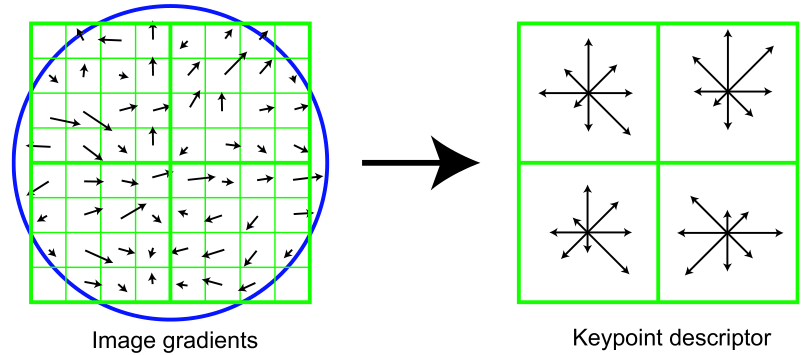
\includegraphics[width=\textwidth]{pictures/SiftGradient.png}
    \caption{Построение дескриптора ключевой точки в методе SIFT}
    \label{fig:sift_gradient}
\end{figure}

Здесь схематично показана часть изображения (слева) и (справа) полученный на её основе дескриптор. Для начала посмотрим налево. Здесь вы можете видеть пиксели, обозначенные маленькими квадратиками. Эти пиксели берутся из квадратного окна дескриптора, которое в свою очередь поделено ещё на четыре равных части (дальше будем называть их регионами). Маленькая стрелочка, в центре каждого пикселя обозначает градиент этого пикселя. Интересно то, что центр этого окна находится между пикселями. Его надо выбирать как можно ближе к точным координатам ключевой точки. Последняя деталь, которую можно увидеть — это круг, обозначающий окно свертки с гауссовым ядром (аналогично окну для вычисления направления ключевой точки). Для этого ядра определяется sigma, равное половине ширины окна дескриптора. В дальнейшем значение каждой точки окна дескриптора будет домножаться на значение гауссова ядра в этой точке, как на весовой коэффициент.

\section{Математические методы}
Помимо системы внешнешнего локального позиционирования, требовалось реализовать систему автономного локального позиционарования по отношению к роботу. Для этого было решено использовать камеру, установленную на роботе и направленную вниз. Определение смещения робота будет происходить при помощи отслеживания смещения изображения между кадрами. Необходимо учесть, что эта система будет работать на роботе, количество вычислительных ресурсов на котором сильно ограничено.

Рассмотрев множество возможных алгоримтов я решил начать воспользоваться самым простым в реализации - полным перебором, а затем попытаться его оптимизировать.

Суть метода заключается в том, что мы запоминаем изображение нашего начального положения, а затем в последующих кадрах, перебирая все возможные смещения, пытаемся наложить изображение друг на друга таким образом, чтобы они были максимально похожи друг на рдруга. Для того чтобы это стало возможным, поверхность, на которой передвигается робот, должна иметь неоднородный рисунок с явно выделяющимися угловыми точками. 

Определим наше изображение через квадратную матрицу размером $N~\times~N$:

\begin{equation}
\begin{pmatrix}
\label{eq:mat_a}
\alpha_{11}& \alpha_{11}& \dots& \alpha_{N1} \\
\alpha_{12}& \alpha_{22}& \dots& \alpha_{N2} \\
\vdots& \vdots& \ddots& \vdots \\
\alpha_{1N}& \alpha_{2N}& \dots& \alpha_{NN}
\end{pmatrix}
\end{equation}

Где $\alpha_{ij} \in [0,255]$ - коэффициент яркости пикселя по кординатам $(i,j)$. 

Назовем матрицей $A$ - изображение начальной позиции робота, матрицей $B$ - изображение последующей позиции робота. Так как робот в пространстве может осуществлять прямолинейное движение и поворот. То и второе изображение будет результатом применения к первому некоторого афинного преобразования - смещения и поворта. Изменение масштаба в данном случае исключено, т. к. расстоение от камеры до снимаемой поверхности - константно. 

Таким образом нашей задачей является - найти соответствующее преобразование из изображения начальной позиции в конечную.

Определим преобразование следующим соотношением:
\begin{equation}
    \begin{array}{c}
        x = x_0 + X [\cos \theta] - [\sin \theta] \\
        y = y_0 + Y [\sin \theta] + [\cos \theta]
    \end{array}
    \label{eq:transform}
\end{equation}

Где $x_0$ и $y_0$ координаты смещения в пикселях, $\theta$ - угол поворота, $X,Y$ - координаты пикселя в начальном изображении.

Таким образом, в результате такого преобразования, элемент $\alpha_{x,y}$ из матрицы (\ref{eq:mat_a}) становится равным элементу матрицы $\alpha_{x_0+X[\cos \theta]-[\sin \theta],~y_0+Y[\sin \theta]+[\cos \theta]}$. В случае если координаты элемента не удволетворяют условию $0\leq,y\leq N$, то считать элемент равным нулю.

В качестве метода интерполяции был использован метод ближейшего соседа.

Определим на обоих изображениях окно, в пределах которых будет происходить поиск преобразования.
Зададим его размер через $k$, где $0 < k < \frac{N}{2}$, а положение внутри через отступы $(i,j)$ относительно центра, где $0 \leq i,j \leq N-\sqrt{2k}$.

Определим функцию $\gamma(A, k, i, j, \theta)$, которая для заданной матрицы $A$ возвращает подматрицу $A^*$ размером $k \times k$, со смещением по координатам $(i,j)$ и поворотом на угол $\theta$ относительно центра в соответствии с преобразованием (\ref{eq:transform}).

За $R^*$ обозначим множество векторов на которых определена функция $\gamma(A,k,x),x\in R^*$.
\begin{equation}
    \{(i,j,\theta):i,j\in \mathbb{Z}, \theta \in \mathbb{R}, 0 \leq i,j \leq N-\sqrt{2k}, -\pi \leq \theta \leq \pi\}
\end{equation}

Чем ближе наше подобранное преобразование к существующему, тем больше полученные изображения будут похожи друг на друга. Степень "похожести"  определим через норму $L_2$ разности матриц $A$ и $B$.

\begin{equation}
    \|A-B\|_2
    \label{eq:delta}
\end{equation}

Обозначим за $\omega$ - вектор $\in$ $R^*$, такой, что: 
\begin{equation}
    \forall x \in R^*\ \Rightarrow \\ \|\gamma(A,k,\omega)-\gamma(B,k,0,0,0)\|_2 \leq \|\gamma(A,k,x)-\gamma(B,k,0,0,0)\|_2 
\end{equation}
Таким образом, $\omega$ - такое преобразование, которое исходное изображение $A$ преобразует в некоторое изображение $A^*$ наиболее похожее на изображение $B^*$, степень похожести который определена через (\ref{eq:delta}).  

Поиск этого преобразования можно осуществлять, например, методом полного перебора. Но перед этим, попробуем построить график функции 
\begin{equation}
    \delta(x,y)=\|\gamma(A,k,x,y,0)-\gamma(B,k,0,0,0)\|_2
\end{equation}
В качестве тестовых, возьмем следующие два изображения:

\begin{figure}[H]
    \begin{tabular}{cc}
        
\includegraphics[width=7cm]{pictures/img1.jpg}
        & 
        
\includegraphics[width=7cm]{pictures/img2.jpg}
    \end{tabular}
    \caption{Изображения начальной и последующей позиций}
\end{figure}

График функции для этих двух изображений будет выглядеть следующим образом:

\begin{figure}[H]
    \centering
    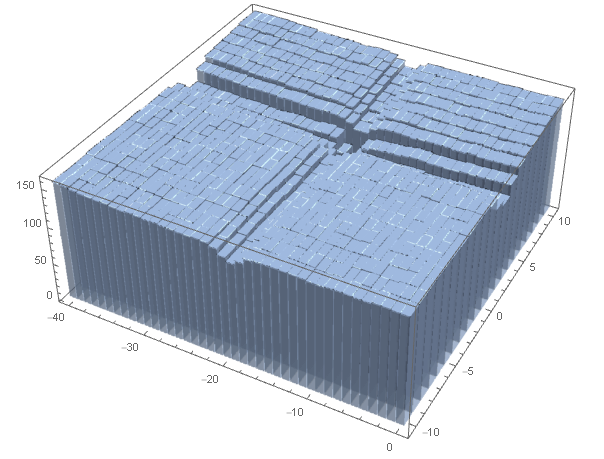
\includegraphics[width=10cm]{pictures/Graphic1.png}
    \caption{График функции разности двух изображений.}
    \label{fig:graphic_delta} 
\end{figure}

На графике (\ref{fig:graphic_delta}) виден минимум функции в точке $(-21,3)$, если наложить два изображения друг на друга с заданным смещением по осям $x$ и $y$ соответсвенно, то их разность будет минимальна. То есть искомое преобразование в данном случае - (-21, 3, 0). На данном этапе мы не будем брать в расчет поворот изображения. 

График функции наталкивает на использование метода градиентного спуска для оптимизации поиска минимума функции. Однако в текущем виде, использование градиентного спуска будет затруднено, т.к. почти на всем пространстве, функция принимает примерно одно и то же значение. Для того чтобы увеличить окрестность вокруг точки минимума, в которой функция заметно уменьшается, можно применить размытие изображений.

Для этого воспользуемся размытием по Гауссу. 

\begin{equation}
    \beta_{i,j}=\frac{1}{2\pi r^2}\sum\limits_{u,v} e^\frac{-(u^2+v^2)}{2r^2} \alpha_{i+u,j+v}
\end{equation}

Где $u$ и $v$ можно выбирать как плюс минус несколько сигм, т.е. радиусов $r$. Радиус размытия подбирается эмпирическим путем.

Оператор, выполняющий размытие по гауссу для изображения $A$ с радиусом $r$ обозначим как $\Gamma(A,r)$

Снова построим график функции разности изображений, но теперь с применением размытия.

\begin{equation}
    \delta(x,y)=\|\Gamma(\gamma(A,k,x,y,0),r)-\Gamma(\gamma(B,k,0,0,0),r)\|_2
\end{equation}

\begin{figure}[H]
    \centering
    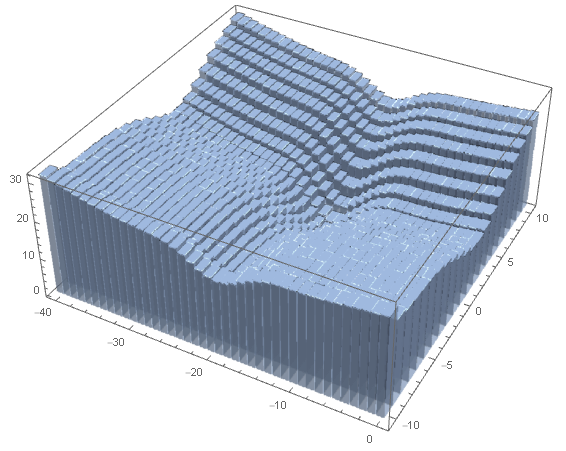
\includegraphics[width=10cm]{pictures/Graphic2.png}
    \caption{График функции разности двух изображений после применения размытия}
    \label{fig:graphic_delta_blur} 
\end{figure}

Как видно на рис. \ref{fig:graphic_delta_blur}, график функции стал более плавным, и спуск заметен на всем пространстве где определена функция, что позволяет применить метод градиентного спуска для поиска минимума. 

Шаг градиентного спуска выбран костантным и подбирается эмпирически. 

При тестировании алгоритма возникала ситуация, когда функция имела несколько точек экстремума, и градиентный спуск сходился к локальному, но не глобальному минимуму. В таком случае было решено в качестве начального приближения использовать результат вычислений на предыдущем кадре, если предположить что временная разница между снимками достаточно мала, и следовательно смещение второго изображения относительного первого достаточно мало, чтобы начальное приближение было близко к искомому минимуму функции. 

\begin{table}[H]
    \centering
    \begin{tabular}{|l|c|}
        \hline
        Алгоритм & Время \\
        \hline
        Полный перебор & 1.278с \\
        \hline
        Градиентный спуск & 0.372c \\
        \hline
        Градиентный спуск + начальное приближение & 0.023с  \\
        \hline
    \end{tabular}
    \caption{Замеры скорости выполнения}
    \label{tab:gradient_time}
\end{table}

Результат работы алгоритма градиентного спуск с использованием начального приближения для ускорения сходимости удовлетворяет нашим требованиям, а именно обеспечения скорости работы как минимум 30 кадров в секунду. В данном случае алгоритм обеспечивает частоту в 43 кадра в секунду, при этом он достаточно стабилен, то есть алгоритм продолжает верно определять смещение на протяжении до 5 минут, при отсутствии резких скачков скорости.

\section{Обзор операционных систем и фреймворков для роботов}

\subsection{Ubuntu Core}
Ubuntu Core служит основой для запуска дополнительных компонентов и приложений, которые оформляются в виде самодостаточных надстроек в формате snap. Компоненты Ubuntu Core, включая базовую систему, ядро Linux и системные надстройки, также поставляются в формате snap и управляются инструментарием snapd. Технология Snappy даёт возможность сформировать образ системы как единое целое, без разбиения на отдельные пакеты.

Вместо поэтапного обновления на уровне отдельных deb-пакетов в Ubuntu Core применяется механизм атомарного обновления snap-пакетов и базовой системы, по аналогии с Atomic, ChromeOS, Endless, CoreOS и Fedora Silverblue. При обновлении базового окружения и snap-пакетов имеется возможность отката состояния до прошлой версии, в случае проблем, выявленных после обновления. В настоящее время в каталоге SnapCraft насчитывается более 4600 snap-пакетов.

Для обеспечения безопасности каждый компонент системы верифицируется по цифровой подписи, что позволяет защитить дистрибутив от внесения скрытых модификаций или установки непроверенных snap-пакетов. Поставляемые в формате Span компоненты изолируются при помощи AppArmor и Seccomp, что создаёт дополнительный рубеж для защиты системы в случае компрометации отдельных приложений. Базовая система включает только минимальный набор необходимых приложений, что не только позволило уменьшить размер системного окружения, но и положительно сказалось на безопасности за счёт уменьшения возможных векторов для атак.

Базовая файловая система монтируется в режиме только для чтения. Обновления выпускаются регулярно, доставляются в режиме ОТА (over-the-air) и синхронизированы с составом Ubuntu 18.04. Для минимизации трафика обновления поставляются в сжатом виде и включают только изменения, относительно прошлого обновления (delta-обновления). Автоматизация установки обновлений решает проблемы с поддержанием безопасности системы при использовании на встраиваемых устройствах.

Благодаря логическому отделению базовой системы от приложений, поддержанием кодовой базы Ubuntu Core в актуальном виде занимаются разработчики Ubuntu, а об актуальности дополнительных приложений заботятся их разработчики. Подобный подход позволяет снизить затраты на сопровождение продуктов, программное окружение которых построено на основе Ubuntu Core, так как их производителям не требуется заниматься выпуском и доставкой системных обновлений и достаточно сосредоточить внимание только на своих специфичных компонентах. 

\subsection{Windows 10 IoT Core}
Windows 10 IoT Core - это версия Windows 10, оптимизированная для небольших устройств с дисплеем или без него, который работает на устройствах ARM и x86 / x64.

Разработчику доступны все приложения платформы Windows, а разработка таких приложений ведется так же, как и любых других приложений и инструментов из Visual Studio, с использованием технологий \verb\C#/XAML\, \verb\HTML/JS\ и др, что означает возможность разработки универсального приложения, которое будет с равным успехом (конечно, учитывая наличие или отсутствие привязки к какой-то специфичной функциональности) работать на PC, телефонах, Xbox или платах. 
\begin{itemize}
    \item IoT Core поддерживает Universal Platform API, включая Universal Drivers, и это является на данный момент основным методом разработки (\verb\C#/C++/JavaScript/HTML/XAML/DirectX\). При этом поддерживаются консольные приложения (\verb\C/C++\);
    \item Отсутствует Windows desktop и командная строка. Но есть Powershell Remoting и SSH;
    \item IoT Core содержит расширения API:
    \begin{itemize}
        \item GPIO, I2C, SPI, ADC, PWM, UART, AllJoyn
        \item Управление системными настройками (язык и др.)
        \item API Set
    \end{itemize}
    \item Веб-сервер Node.js с используемым внутри Microsoft Chakra.
\end{itemize}

Однако необходимо учитывать отсутствие драйверов и поддержки для некоторых модулей (например, Wi-Fi), что блокирует часть сценариев.

На Windows 10 IoT Core создают, например, хабы для домашних устройств. При условии того, что правильным образом будет использована встроенная функциональность AllJoyn, можно управлять окружающими устройствами. То есть быть управляющей панелью, собирая данные с сенсоров и других устройств. 
Таким образом, теперь у разработчиков есть выбор – можно продолжать использовать всё то, что уже разработано на OSS, и подключать при необходимости облако для обработки данных, либо взять знакомые инструменты (Visual Studio, .NET) и создать универсальное приложение. 

\subsection{Robot Operating System}
Robot Operating System (ROS) - это гибкая среда для написания программного обеспечения для роботов. Это набор инструментов, библиотек и соглашений, призванных упростить задачу создания сложного и надежного поведения робота на самых разных роботизированных платформах.

С точки зрения робота, проблемы, которые кажутся человеку тривиальными, часто сильно различаются между экземплярами задач и сред. Работать с этими вариациями так сложно, что ни один человек, лаборатория или учреждение не могут надеяться сделать это самостоятельно.

ROS был создан с нуля, чтобы стимулировать совместную разработку программного обеспечения для робототехники. Например, одна лаборатория может иметь экспертов по составлению карт в помещениях и может предложить систему мирового класса для создания карт. Другая группа могла бы иметь экспертов по использованию карт для навигации, а другая группа могла бы обнаружить подход компьютерного зрения, который хорошо работает для распознавания небольших объектов в беспорядке. 
На самом низком уровне ROS предлагает интерфейс передачи сообщений, который обеспечивает межпроцессное взаимодействие и обычно называется промежуточным программным обеспечением.

Промежуточное программное обеспечение ROS предоставляет следующие возможности:
\begin{itemize}
    \item публиковать / подписывать анонимные сообщения
    \item запись и воспроизведение сообщений
    \item запрос / ответ удаленных вызовов процедур
    \item система с распределенными параметрами
\end{itemize}

Передача сообщений:
Система связи часто является одной из первых потребностей, возникающих при реализации нового приложения робота. Встроенная и хорошо протестированная система обмена сообщениями ROS экономит ваше время, управляя деталями взаимодействия между распределенными узлами посредством анонимного механизма публикации / подписки. Другое преимущество использования системы передачи сообщений заключается в том, что она заставляет вас реализовывать четкие интерфейсы между узлами в вашей системе, тем самым улучшая инкапсуляцию и способствуя повторному использованию кода. Структура этих интерфейсов сообщений определяется в сообщении IDL (Язык описания интерфейса).

Запись и воспроизведение сообщений:
Поскольку система публикации / подписки является анонимной и асинхронной, данные могут быть легко получены и воспроизведены без каких-либо изменений в коде. Допустим, у вас есть задача A, которая считывает данные с датчика, и вы разрабатываете задачу B, которая обрабатывает данные, полученные с помощью задачи A. ROS упрощает сбор данных, опубликованных с помощью задачи A, в файл, а затем повторно публикует эти данные из файл позже. Абстракция передачи сообщений позволяет задаче B быть независимой от источника данных, который может быть задачей A или файлом журнала. Это мощный шаблон проектирования, который может значительно сократить усилия по разработке и повысить гибкость и модульность системы.

Удаленные вызовы процедур:
Асинхронный характер обмена сообщениями «публикация / подписка» работает для многих коммуникационных потребностей в робототехнике, но иногда требуется синхронное взаимодействие между запросами и ответами. Промежуточное программное обеспечение ROS предоставляет эту возможность с помощью служб. Подобно темам, данные, передаваемые между процессами в вызове службы, определяются с помощью одного и того же простого сообщения IDL.

Система распределенных параметров:
Промежуточное программное обеспечение ROS также позволяет задачам обмениваться информацией о конфигурации через глобальное хранилище значений ключей. Эта система позволяет легко изменять настройки задач и даже позволяет задачам изменять конфигурацию других задач.

\subsection{FreeRTOS}
FreeRTOS — многозадачная операционная система реального времени (ОСРВ) для встраиваемых систем. Портирована на 35 микропроцессорных архитектур. 

Операционная система реального времени FreeRTOS рассчитана на работу в таких, задаваемых особенностями массовых микроконтроллеров, условиях, как низкое быстродействие аппаратуры и малый объём оперативной памяти, отсутствие поддержки на аппаратном уровне таких механизмов операционных систем, как блок управления памятью (MMU) и механизмы реализации многозадачности, такие, как быстрое переключение контекста.

Начиная с версии 4, FreeRTOS позволяет использовать сопрограммы — задачи, использующие невытесняющую многозадачность и требующие очень мало оперативной памяти для запуска.

Диспетчер (англ. scheduler) системы очень маленький (занимает, в зависимости от платформы и настроек ядра, 4-9 килобайт) и простой, однако позволяет задать различные приоритеты процессов, вытесняющую и невытесняющую многозадачность, семафоры и очереди.

Список преимуществ:
\begin{itemize}
    \item Предоставляет единое и независимое решение для множества различных архитектур и инструментов разработки.
    \item Надежный. Доверие обеспечивается деятельностью, предпринятой родственным проектом SafeRTOS.
    \item Является многофункциональным и все еще находится в процессе постоянного активного развития.
    \item Имеет минимальное ПЗУ, ОЗУ и накладные расходы на обработку. Обычно двоичное изображение ядра RTOS будет иметь размер от 6 до 12 Кбайт.
    \item Ядро RTOS содержится только в 3 файлах С. 
    \item Имеет путь перехода к SafeRTOS, который включает сертификаты для медицинского, автомобильного и промышленного секторов.
    \item Хорошо зарекомендовал себя с большой и постоянно растущей пользовательской базой.
    \item Содержит предварительно настроенный пример для каждого порта.
    \item FreeRTOS предлагает меньшую и более простую альтернативу обработки в реальном времени для приложений, в которых eCOS, встроенный Linux (или Real Time Linux) и даже uCLinux не подходят или недоступны.
\end{itemize}

\subsection{Сравнение}

\begin{table}[H]
    \centering
    \begin{tabular}{|p{4cm}|c|c|c|c|}
    \hline
    Возможность / ОС & Windows 10 Core & Ubuntu Core & FreeRTOS & ROS \\
    \hline
    Многозадачность & - & + & + & + \\
    \hline
    Работа в реальном времени & - & - & + & - \\
    \hline
    Файловая система  & - & + & + & + \\
    \hline
    Многопоточность & + & + & + & + \\
    \hline
    Драйверы работы с сетью & + & + & - & + \\
    \hline
    \end{tabular}
    \caption{Сравнительная таблица возможностей операционных систем для роботов}
    \label{tab:os_summarize}
\end{table}

Посмотрев на предоставляемые возможности (см. табл.~\ref{tab:os_summarize}) выделенных операционных систем было решено использовать ROS. К ПО на роботе нет требований к работе в реальном времени, соответсвенно такие ОС как FreeRTOS можно отмести, они все еще хороши тем, что довольно быстры и не требовательны к ресурсам. Однако другие операционные системы предоставляют больший список возможностей. ROS представляет из себя не операционную систему а целый фреймворк для написания ПО для роботов и разрабатывался для операционной системы Linux. Его возможно запускать и на Windows но только используя возможности виртуализации, такие как например Docker \cite{web:docker}. Но последнее невозможно сделать на операционной системе Windows IoT Core, а ставить другие операционные системы на одноплатные компьютеры, где не предполагается использовать интерфейс является нецелесообразным. Поэтому было решено возпользоваться связкой Ubuntu Core + ROS. ROS в связи со своей архитектурой позволяет производить обмен сообщениями не только в пределах локальной машины, но так же и по сети. Что, например, позволит вынести часть требовательных к производительности функций с робота на сервер, и производить управление роботом используя уже существующий протокол передачи сообщений.

\section{Заключение}
В ходе работы была успешно реализована система автоматического управления соревнованиями роботов RATS.
В ходе работы было:
\begin{itemize}
    \item Написано 7250 строк кода на PHP.
    \item Написано 400 строк кода на языке шаблонизатора Blade.
    \item Написано 1500 строк кода С++.
    \item Сделано более 100 коммитов.
\end{itemize}

\newpage
\bibliographystyle{utf8gost705u} 
\bibliography{lib.bib} 

\end{document}
